\documentclass{beamer}

\usefonttheme{professionalfonts} % using non standard fonts for beamer
\usefonttheme{serif} % default family is serif

\usepackage{hyperref}

%\usepackage{minted}

\usepackage{animate}

\usepackage{graphicx}

\def\Put(#1,#2)#3{\leavevmode\makebox(0,0){\put(#1,#2){#3}}}

\usepackage{color}

\usepackage{tikz}

\usepackage{amssymb}
\usepackage{amsthm}

\usepackage{enumerate}


\newcommand\blfootnote[1]{%

  \begingroup

  \renewcommand\thefootnote{}\footnote{#1}%

  \addtocounter{footnote}{-1}%

  \endgroup

}

\makeatletter

%%%%%%%%%%%%%%%%%%%%%%%%%%%%%% Textclass specific LaTeX commands.

 % this default might be overridden by plain title style

 \newcommand\makebeamertitle{\frame{\maketitle}}%

 % (ERT) argument for the TOC

 \AtBeginDocument{%

   \let\origtableofcontents=\tableofcontents

   \def\tableofcontents{\@ifnextchar[{\origtableofcontents}{\gobbletableofcontents}}

   \def\gobbletableofcontents#1{\origtableofcontents}

 }

%%%%%%%%%%%%%%%%%%%%%%%%%%%%%% User specified LaTeX commands.

\usetheme{Malmoe}

% or ...

\useoutertheme{infolines}

\addtobeamertemplate{headline}{}{\vskip2pt}

\setbeamertemplate{theorems}[numbered]

\theoremstyle{definition}
\newtheorem{defn}{Definition}[section]

\setbeamercovered{transparent}

% or whatever (possibly just delete it)

\makeatother

\begin{document}
\title[Discussion 9]{CS/MATH 111, Discrete Structures - Fall 2018. \\ Discussion 9 - Graphs}
\author[CS111]{Andres, Sara, Elena}
\institute[Fall'18]{University of California, Riverside}
\makebeamertitle
\newif\iflattersubsect

\AtBeginSection[] {
    \begin{frame}<beamer>
    \frametitle{Outline} 
    \tableofcontents[currentsection]  
    \end{frame}
    \lattersubsectfalse
}

\AtBeginSubsection[] {
    \begin{frame}<beamer>
    \frametitle{Outline} 
    \tableofcontents[currentsubsection]  
    \end{frame}
}

\section{Bipartite graph}

\begin{frame}{Bipartite graph}
    \begin{itemize}
        \item A bipartite graph, also called a bigraph, is a set of graph vertices decomposed into two disjoint sets such that no two graph vertices within the same set are adjacent.
        \item Bipartite graphs are equivalent to two-colorable graphs. 
        \item All acyclic graphs are bipartite. 
        \item A cyclic graph is bipartite iff all its cycles are of even length
    \end{itemize}
\end{frame}

\begin{frame}{Bipartite graph}
    \centering 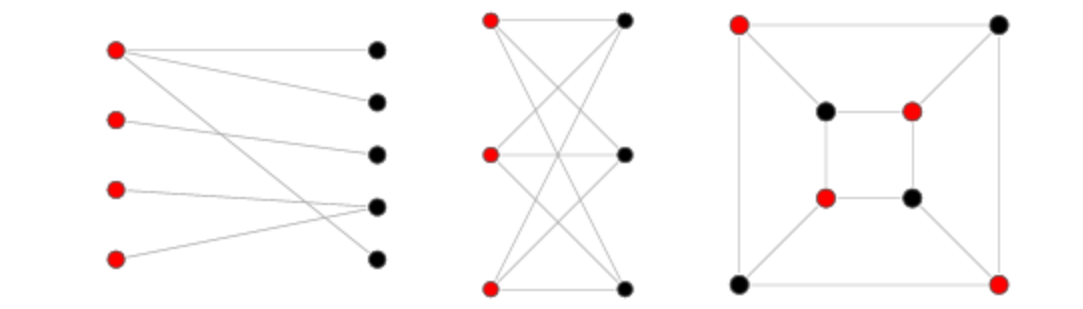
\includegraphics[width=.7\linewidth]{p5.PNG}
\end{frame}

\section{Perfect matching}

\begin{frame}{Perfect matching}
A perfect matching of a graph is a matching (i.e., an independent edge set) in which every vertex of the graph is incident to exactly one edge of the matching. 
\\A perfect matching is therefore a matching containing $\frac{n}{2}$ edges (the largest possible), meaning perfect matchings are only possible on graphs with an even number of vertices.
\end{frame}

\begin{frame}{Perfect matching}
 Hall’s Theorem: Let G = (X,Y ) be a bipartite graph. Then X has a perfect macthing into Y if and only if for all $T \subseteq X$, the inequality $|T| \leq |N(T)|$ holds. Where N(T) is the set of all neighbors of the vertices in T. In other words, $y \in  Y$ is an element of N(T) if and only if there is a vertex $x \in  T$ so that xy is an edge.
\end{frame}

\begin{frame}{Perfect matching}
    \begin{flushleft}
        You are given two bipartite graph G and H below. For each graph determine whether it has a perfect matching. Justify your answer, either by listing the edges that are in the matching or use Hall's Theorem to show that the graph does not have a perfect matching.
    \end{flushleft}
    \centering 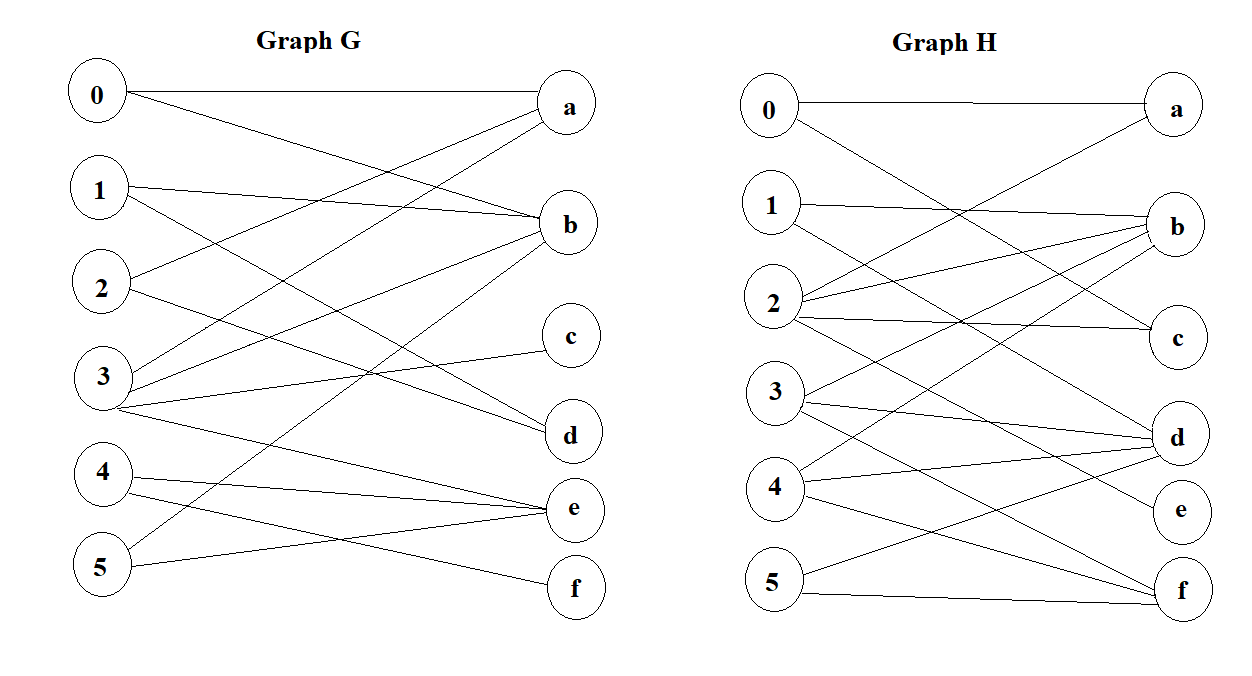
\includegraphics[width=.7\linewidth]{p6.jpg}
\end{frame}

\begin{frame}{Perfect matching}
    \centering 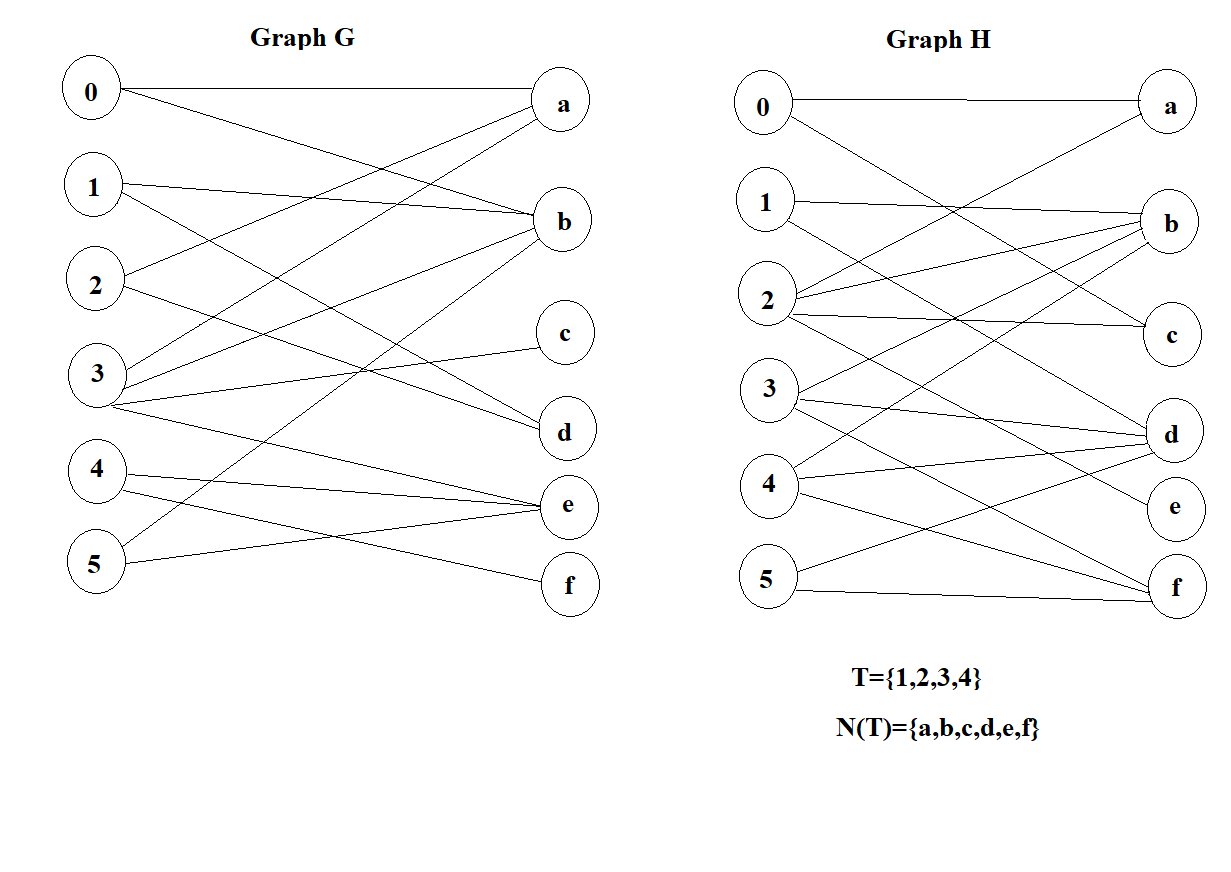
\includegraphics[width=.7\linewidth]{p7.PNG}
\end{frame}

\end{document}
